\section{Introduction}
%\todo[inline]{write introduction}

The virtual creation and perception of real environments or imaginary settings, rendered by a computer, using specialized software, is referred to as virtual reality (VR). Its goal is to simulate a user's physical presence in this environment, by enabling the user to interact with this space and any objects depicted therein using specialized display screens or projectors and other devices.

The potential of virtual reality in gaming is an enormous factor both for the scientific and commercial sector regarding its multitude of use cases. 

In the past decade a variety of electronic devices has reached the marked and found its way into the homes of consumers. Gaming consoles have become entertainment systems offering more than just the gaming aspect. Computers gained the abilities of past supercomputers and are far more than workstations for the majority of modern population. With technological advancements made in the past 50 Years and popularity gains of these systems also the gaming industry has reached its heyday. 

VR, although expensive, gains more interest and the audience grows almost daily. 
Games that do not naturally support VR are searching for ways to include VR in 
their games, some of the problems and advantages are described in the section 
\textit{Games And The Virtual Reality}\ref{sec:gamesNvr}.

\begin{figure}%[h]
	\centering
	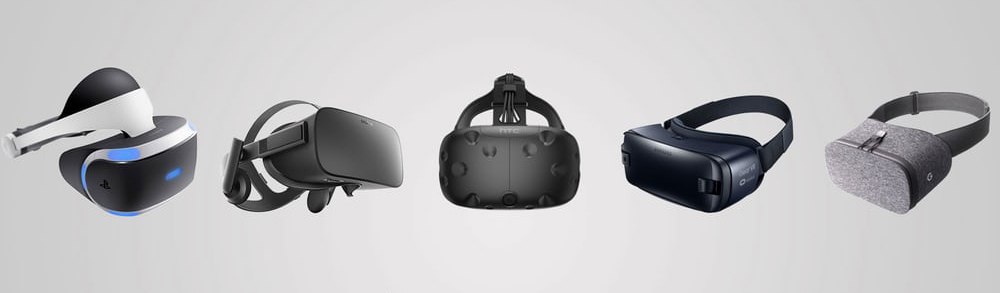
\includegraphics[width=0.99\columnwidth]{./figures/vr-hmd}
	\caption[vr-hmd]{Overview of different consumer HMD as available in late 2016. FLTR Plystation VR, Oculus Rift, HTC Vive, Samsung Gear VR, Daydream View.\footnotemark}~\label{fig:vrHMD}
\end{figure}
\footnotetext{\textcopyright~Newatlas, [Online; accessed January 04., 2017],[Digitally revised] \url{http://img-2.newatlas.com/vr-comparison-2016-b-2.jpg}}

The development of consumer friendly head mounted devices (HMD) for VR, as to see in \textbf{Figure~\ref{fig:vrHMD}}, has just picked up in recent years with systems like the \textit{Oculus Rift in March 2016}, the \textit{HTC Vive in April 2016}, the \textit{Samsung Gear VR in August 2016}, the \textit{Playstation VR in October 2016} or the \textit{Daydream View in November 2016}. 

Many developers have already started to develop games that use the advances of VR and are serving quick. The research on this fields has lacked behind on reliable results regarding the ideal approach to points such as immersion, interaction and performance. This publication intends to show the many disciplines and what research can be done to improve VR in Games.

